%%
%  ******************************************************************************
%  * #file    Szablon_raportu_EN_Latex.tex
%  * #author  Adrian Wójcik   adrian.wojcik(at)put.poznan.pl
%  *          
%  * #commit  Patryk Kościk   koscikpatryk(at)gmail.com
%  *          Modified the template for Projekt przejsciowy purposes          
%  *          
%  *
%  * #commit  Patryk Kościk   koscikpatryk(at)gmail.com
%  *          Zupełnie przewrócono na łeb formatke po taktycznym wyjasnieniu          
%  *          
%  * #version 1.1
%  * #date    09-Mar-2022
%  * #brief   PROJPRZEJ
%  *
%  ******************************************************************************
%%  
\documentclass[11pt, a4paper]{article}

\usepackage{SM_template}

% Wypełnijcie te dyrektywy zgodnie z waszym tematem
%
% \lab      -> NAZWA CZUJNIKA,          np.: 'DHT22'
% \comment  -> Króciutki opis co to,    np.: 'Cyfrowy czujnik temperatury'
% \author   -> Autor dokumentu          np.: Patryk Kościk
%
% Pamiętajcie o zmianie ścieżki w \addbibresourcue (!)

\lab{Moduł HW-487}
\comment{Optyczny czujnik szczelinowy}
\author{Jakub Grzesiak}
\addbibresource{bib/HW-487.bib}

%
% Początek dokumentu
%
\begin{document}

%
% Strona tytułowa
%
\mainpage{HW-487/zdj_modułu/front.jpg}
\newpage

\section*{Opis elementu}
Optyczny czujnik szczelinowy (ang. photo interrupter) to cyfrowy sensor zbudowany z diody emitującej promieniowanie podczerwone (IR LED) oraz fototranzystora, który odbiera sygnał świetlny wysyłany przez tę diodę. Komponenty te umieszczone są po obu stronach obudowy w kształcie litery 'U' w taki sposób, aby możliwa była pomiędzy nimi komunikacja optyczna, co przedstawiono na rysunku (\ref{fig:_zasada_dzialania_elementu}). Czujniki tego typu znajdują zastosowanie w takich urządzeniach jak: drukarki i skanery, enkodery optyczne, przełączniki (switche) optyczne w nowoczesnych klawiaturach czy jako elementy włączników hotelowych, które zamykają obwód oświetlenia w pokoju po umieszczeniu w nich karty.


%%%%%%%%%%%%%%%%%%%%%%%%%  TWO IMAGES SIDE BY SIDE  %%%%%%%%%%%%%%%%%%%%%%%%%%%%%
\vspace{0.25cm}
\begin{figure}[h]
\centering
%%%%%%%%%%%%%%%%%%%%%%%%%%%%%%%%%%%%%%%%%%%%%%%%%%%%%%%%%%%%%%%%%%%%%%%%%%%%%%%%%
\begin{subfigure}{.5\textwidth}
\centering
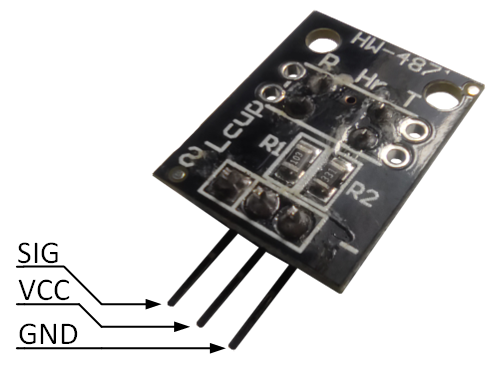
\includegraphics[width=.7\linewidth]{fig/HW-487/zdj_modułu/reverse.png}
\caption{Fizyczna budowa czujnika wraz z pinoutem}
\label{fig:_zdjecie_elementu}
\end{subfigure}%
%%%%%%%%%%%%%%%%%%%%%%%%%%%%%%%%%%%%%%%%%%%%%%%%%%%%%%%%%%%%%%%%%%%%%%%%%%%%%%%%%
\begin{subfigure}{.5\textwidth}
\centering
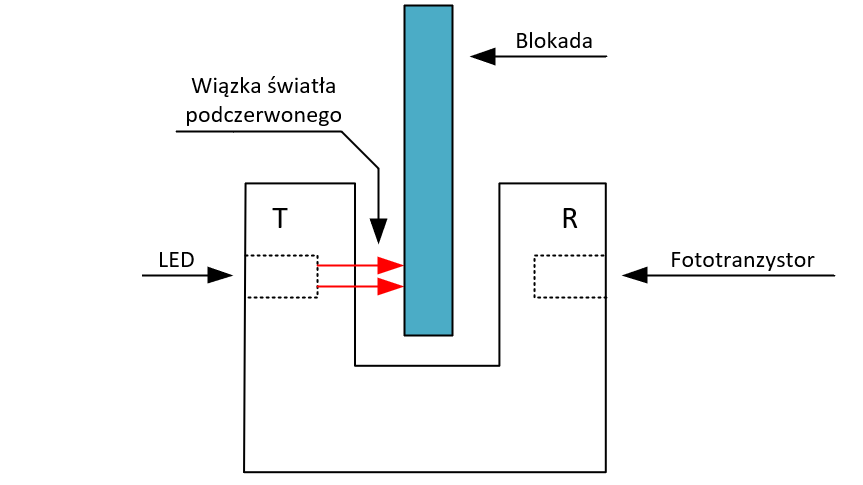
\includegraphics[width=1.05\linewidth]{fig/HW-487/zasada_dzialania/PhotoInterrupter_1.png}
\caption{Schematyczne przedstawienie działania czujnika}
\label{fig:_zasada_dzialania_elementu}
\end{subfigure}
%%%%%%%%%%%%%%%%%%%%%%%%%%%%%%%%%%%%%%%%%%%%%%%%%%%%%%%%%%%%%%%%%%%%%%%%%%%%%%%%%
% \caption{PODPIS}
\label{fig:element}
\end{figure}
\vspace{0.25cm}
%%%%%%%%%%%%%%%%%%%%%%%%%  TWO IMAGES SIDE BY SIDE  %%%%%%%%%%%%%%%%%%%%%%%%%%%%%

% \subsection{Opis modułu} REPLACE SUBSECTION WITH 1CM VSPACE
Czujnik może być zasilany napięciami z zakresu $3,3V - 5V DC$. Schemat budowy wewnętrznej przedstawiono na rysunku (\ref{fig:_schemat_modulu}). Rezystor R2 pełni rolę ogranicznika prądu płynącego przez diodę. Rezystor R1 natomiast jest rezystorem podciągającym na linii sygnałowej. Jest wymagany, aby wyjście S znajdowało się w stanie wysokim, gdy do fototranzystora nie dociera światło z diody. W omawianym czujniku oba rezystory są wlutowane na PCB.

%%%%%%%%%%%%%%%%%%%%%%%%%  TWO IMAGES SIDE BY SIDE  %%%%%%%%%%%%%%%%%%%%%%%%%%%%%
\begin{figure}[h]
\centering
%%%%%%%%%%%%%%%%%%%%%%%%%%%%%%%%%%%%%%%%%%%%%%%%%%%%%%%%%%%%%%%%%%%%%%%%%%%%%%%%%
\begin{subfigure}{.5\textwidth}
\centering
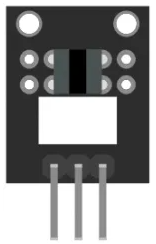
\includegraphics[width=.3\linewidth]{fig/HW-487/zdj_modułu/arduino_modules.png}
\caption{Ilustracja modułu \cite{ArduinoModules:PhotoInterrupter}}
\label{fig:_zdjecie_modulu}
\end{subfigure}%
%%%%%%%%%%%%%%%%%%%%%%%%%%%%%%%%%%%%%%%%%%%%%%%%%%%%%%%%%%%%%%%%%%%%%%%%%%%%%%%%%
\begin{subfigure}{.5\textwidth}
\centering
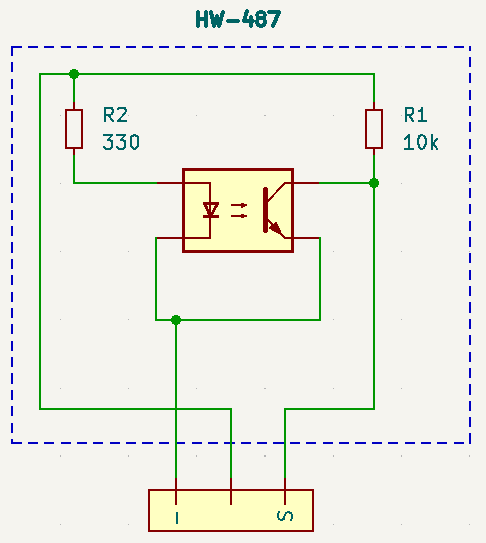
\includegraphics[width=.55\linewidth]{fig/HW-487/polaczenie_modulu/schematics.png}
\caption{Schemat budowy wewnętrznej modułu}
\label{fig:_schemat_modulu}
\end{subfigure}
%%%%%%%%%%%%%%%%%%%%%%%%%%%%%%%%%%%%%%%%%%%%%%%%%%%%%%%%%%%%%%%%%%%%%%%%%%%%%%%%%
\label{fig:modul}
\end{figure}
\vspace{0.25cm}
%%%%%%%%%%%%%%%%%%%%%%%%%  TWO IMAGES SIDE BY SIDE  %%%%%%%%%%%%%%%%%%%%%%%%%%%%%
Zasada działania oparta jest na pracy fototranzystora jako klucza/przełącznika, który przyjmuje dwa stany - zatkania lub nasycenia - w zależności od wiązki światła padającej na jego bazę. Gdy w szczelinie znajduje się przeszkoda - sytuacja przedstawiona na rysunku (\ref{fig:_zasada_dzialania_elementu}) - fototranzystor nie przewodzi (znajduje się w stanie zatkania). Prowadzi to do przepływu prądu od zasilania (pin środkowy - VCC), przez rezystor R1, do wyjścia (pin S - SIG) i wysterowania go w stan wysoki. W przeciwnej sytuacji, gdy na bazę fototranzystora pada wiązka podczerwieni z diody, znajduje się on w stanie nasycenia. Prąd przepływa wtedy od zasilania, przez rezystor R1, fototranzystor, aż do masy (pin ''-'' - GND). Na wyjściu S pojawia się wtedy stan niski.

\newpage

\section{Użycie czujnika}
Czujnik posiada 3 wyprowadzenia - dwa zasilające i jedno sygnałowe. Na rys. \ref{fig:_zdjecie_elementu} przedstawiono oznaczenia wyprowadzeń rzeczywistego czujnika. Działanie czujnika można zweryfikować z użyciem mikrokontrolera. W poniższym przykładzie użyto płytki rozwojowej STM32 NUCLEO-F767ZI. Układ połączeń przedstawiony na rysunku (\ref{fig:_polaczenie_ukladu}) oraz program dla płytki NUCLEO-F746ZG będzie identyczny. Kod skonfigurowano tak, aby po zablokowaniu szczeliny uruchamiana była wbudowana w płytkę mikrokontrolera dioda LD1.

\vspace{0.25cm}
\begin{figure}[h]
    \centering
    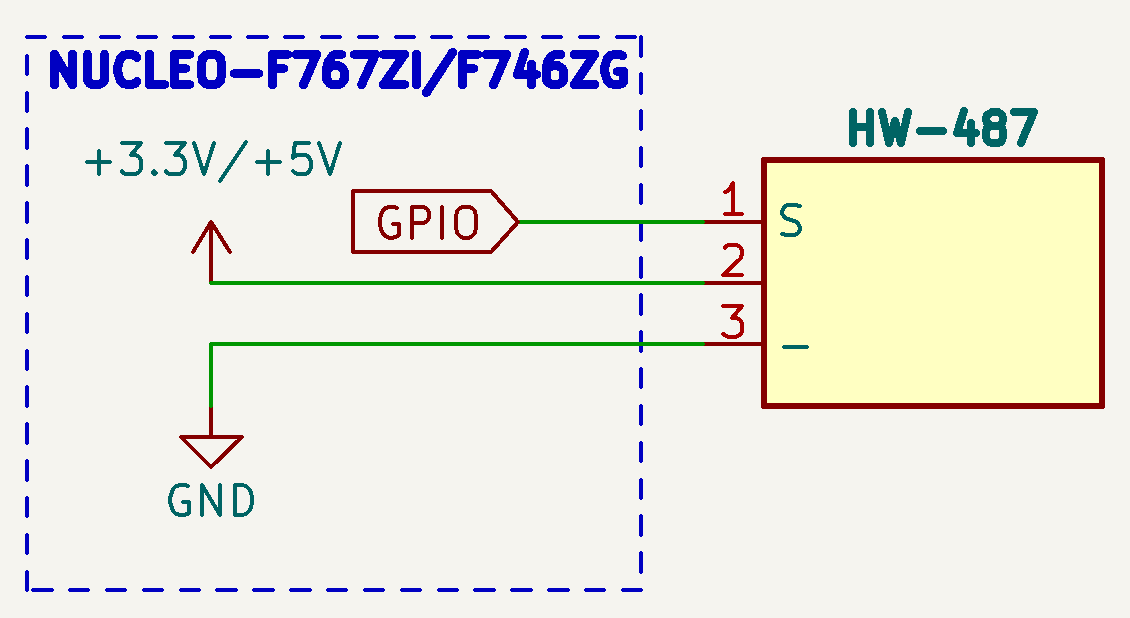
\includegraphics[width=0.6\textwidth]{fig/HW-487/polaczenie_modulu/nucleo_con_v2.png}
    \caption{Połączenie układu z mikroprocesorem}
    \label{fig:_polaczenie_ukladu}
\end{figure}
\vspace{0.25cm}

Poniżej zaprezentowano zdjęcia rzeczywistego układu w dwóch stanach. Konfiguracja pliku \texttt{.IOC} i kod zawarte są w \texttt{Suplement \#1}.

% TUTAJ FOTY ODNOSNIE TEGO
%%%%%%%%%%%%%%%%%%%%%%%%%  TWO IMAGES SIDE BY SIDE  %%%%%%%%%%%%%%%%%%%%%%%%%%%%%
\vspace{0.25cm}
\begin{figure}[h]
\centering
%%%%%%%%%%%%%%%%%%%%%%%%%%%%%%%%%%%%%%%%%%%%%%%%%%%%%%%%%%%%%%%%%%%%%%%%%%%%%%%%%
\begin{subfigure}{.5\textwidth}
\centering
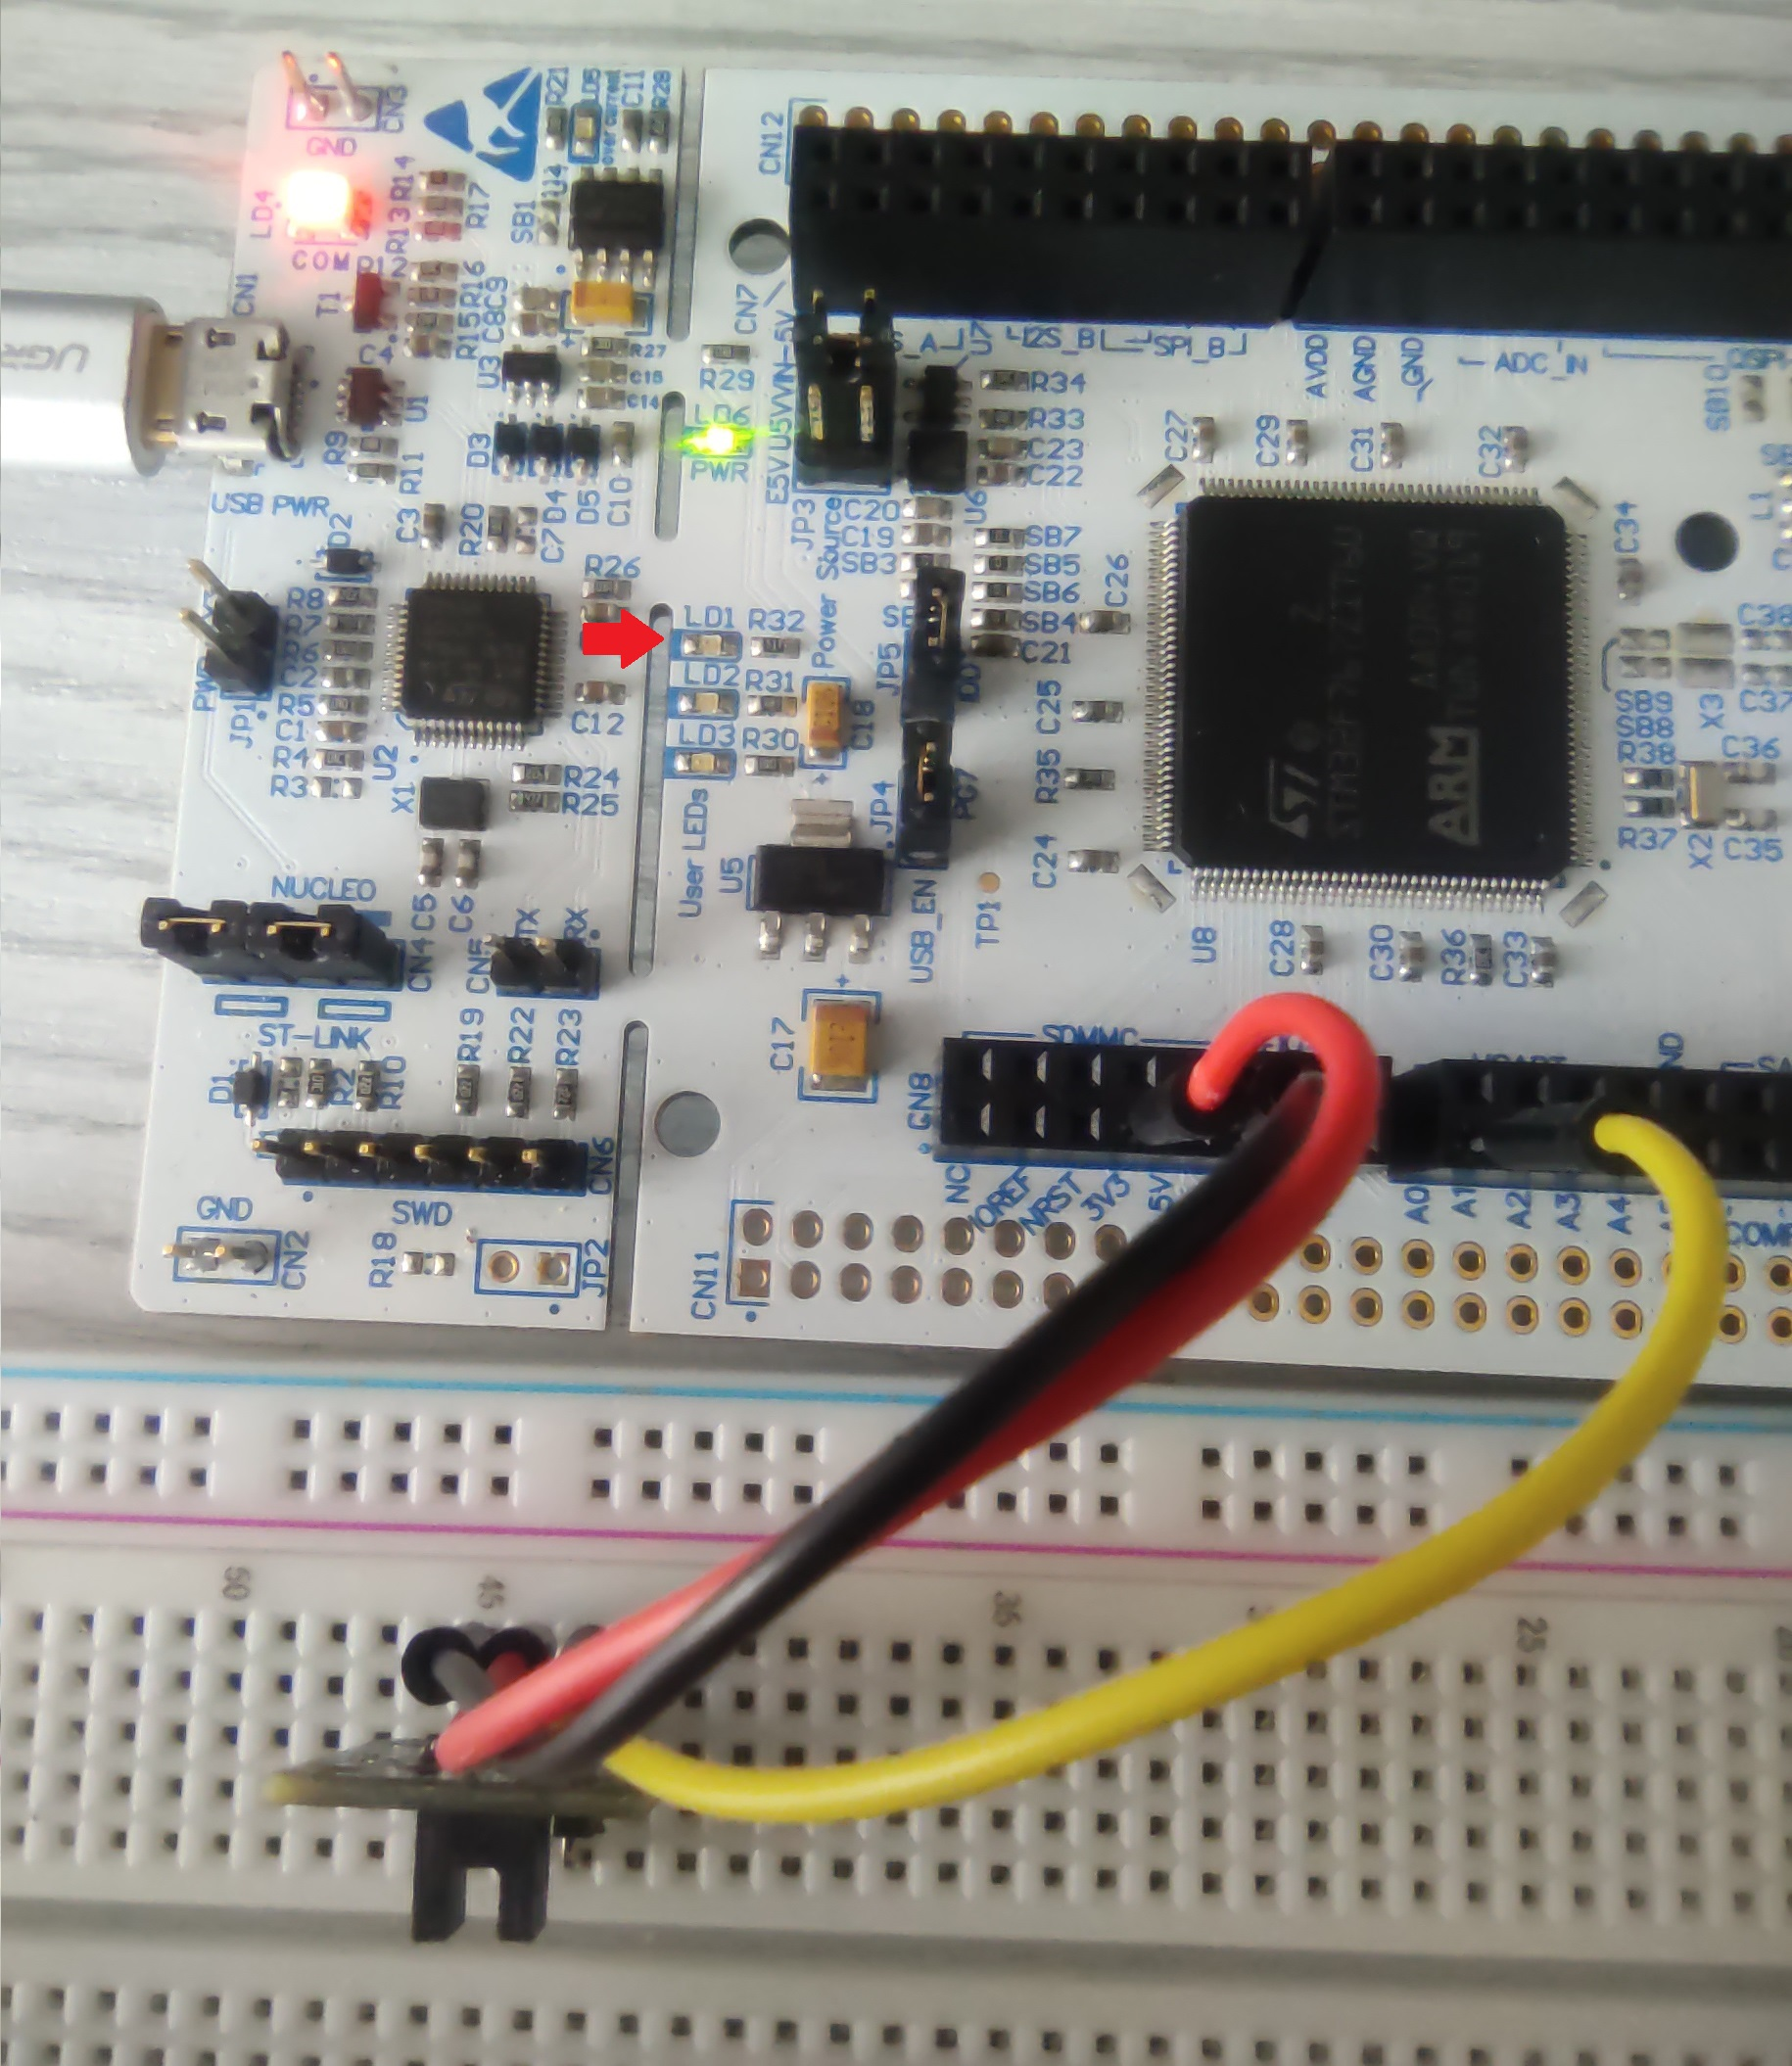
\includegraphics[width=.76\linewidth]{fig/HW-487/działanie_ukladu/led_off.jpg}
\caption{Szczelina pusta - stan niski na wyjściu S}
\label{fig:_uklad_off}
\end{subfigure}%
%%%%%%%%%%%%%%%%%%%%%%%%%%%%%%%%%%%%%%%%%%%%%%%%%%%%%%%%%%%%%%%%%%%%%%%%%%%%%%%%%
\begin{subfigure}{.5\textwidth}
\centering
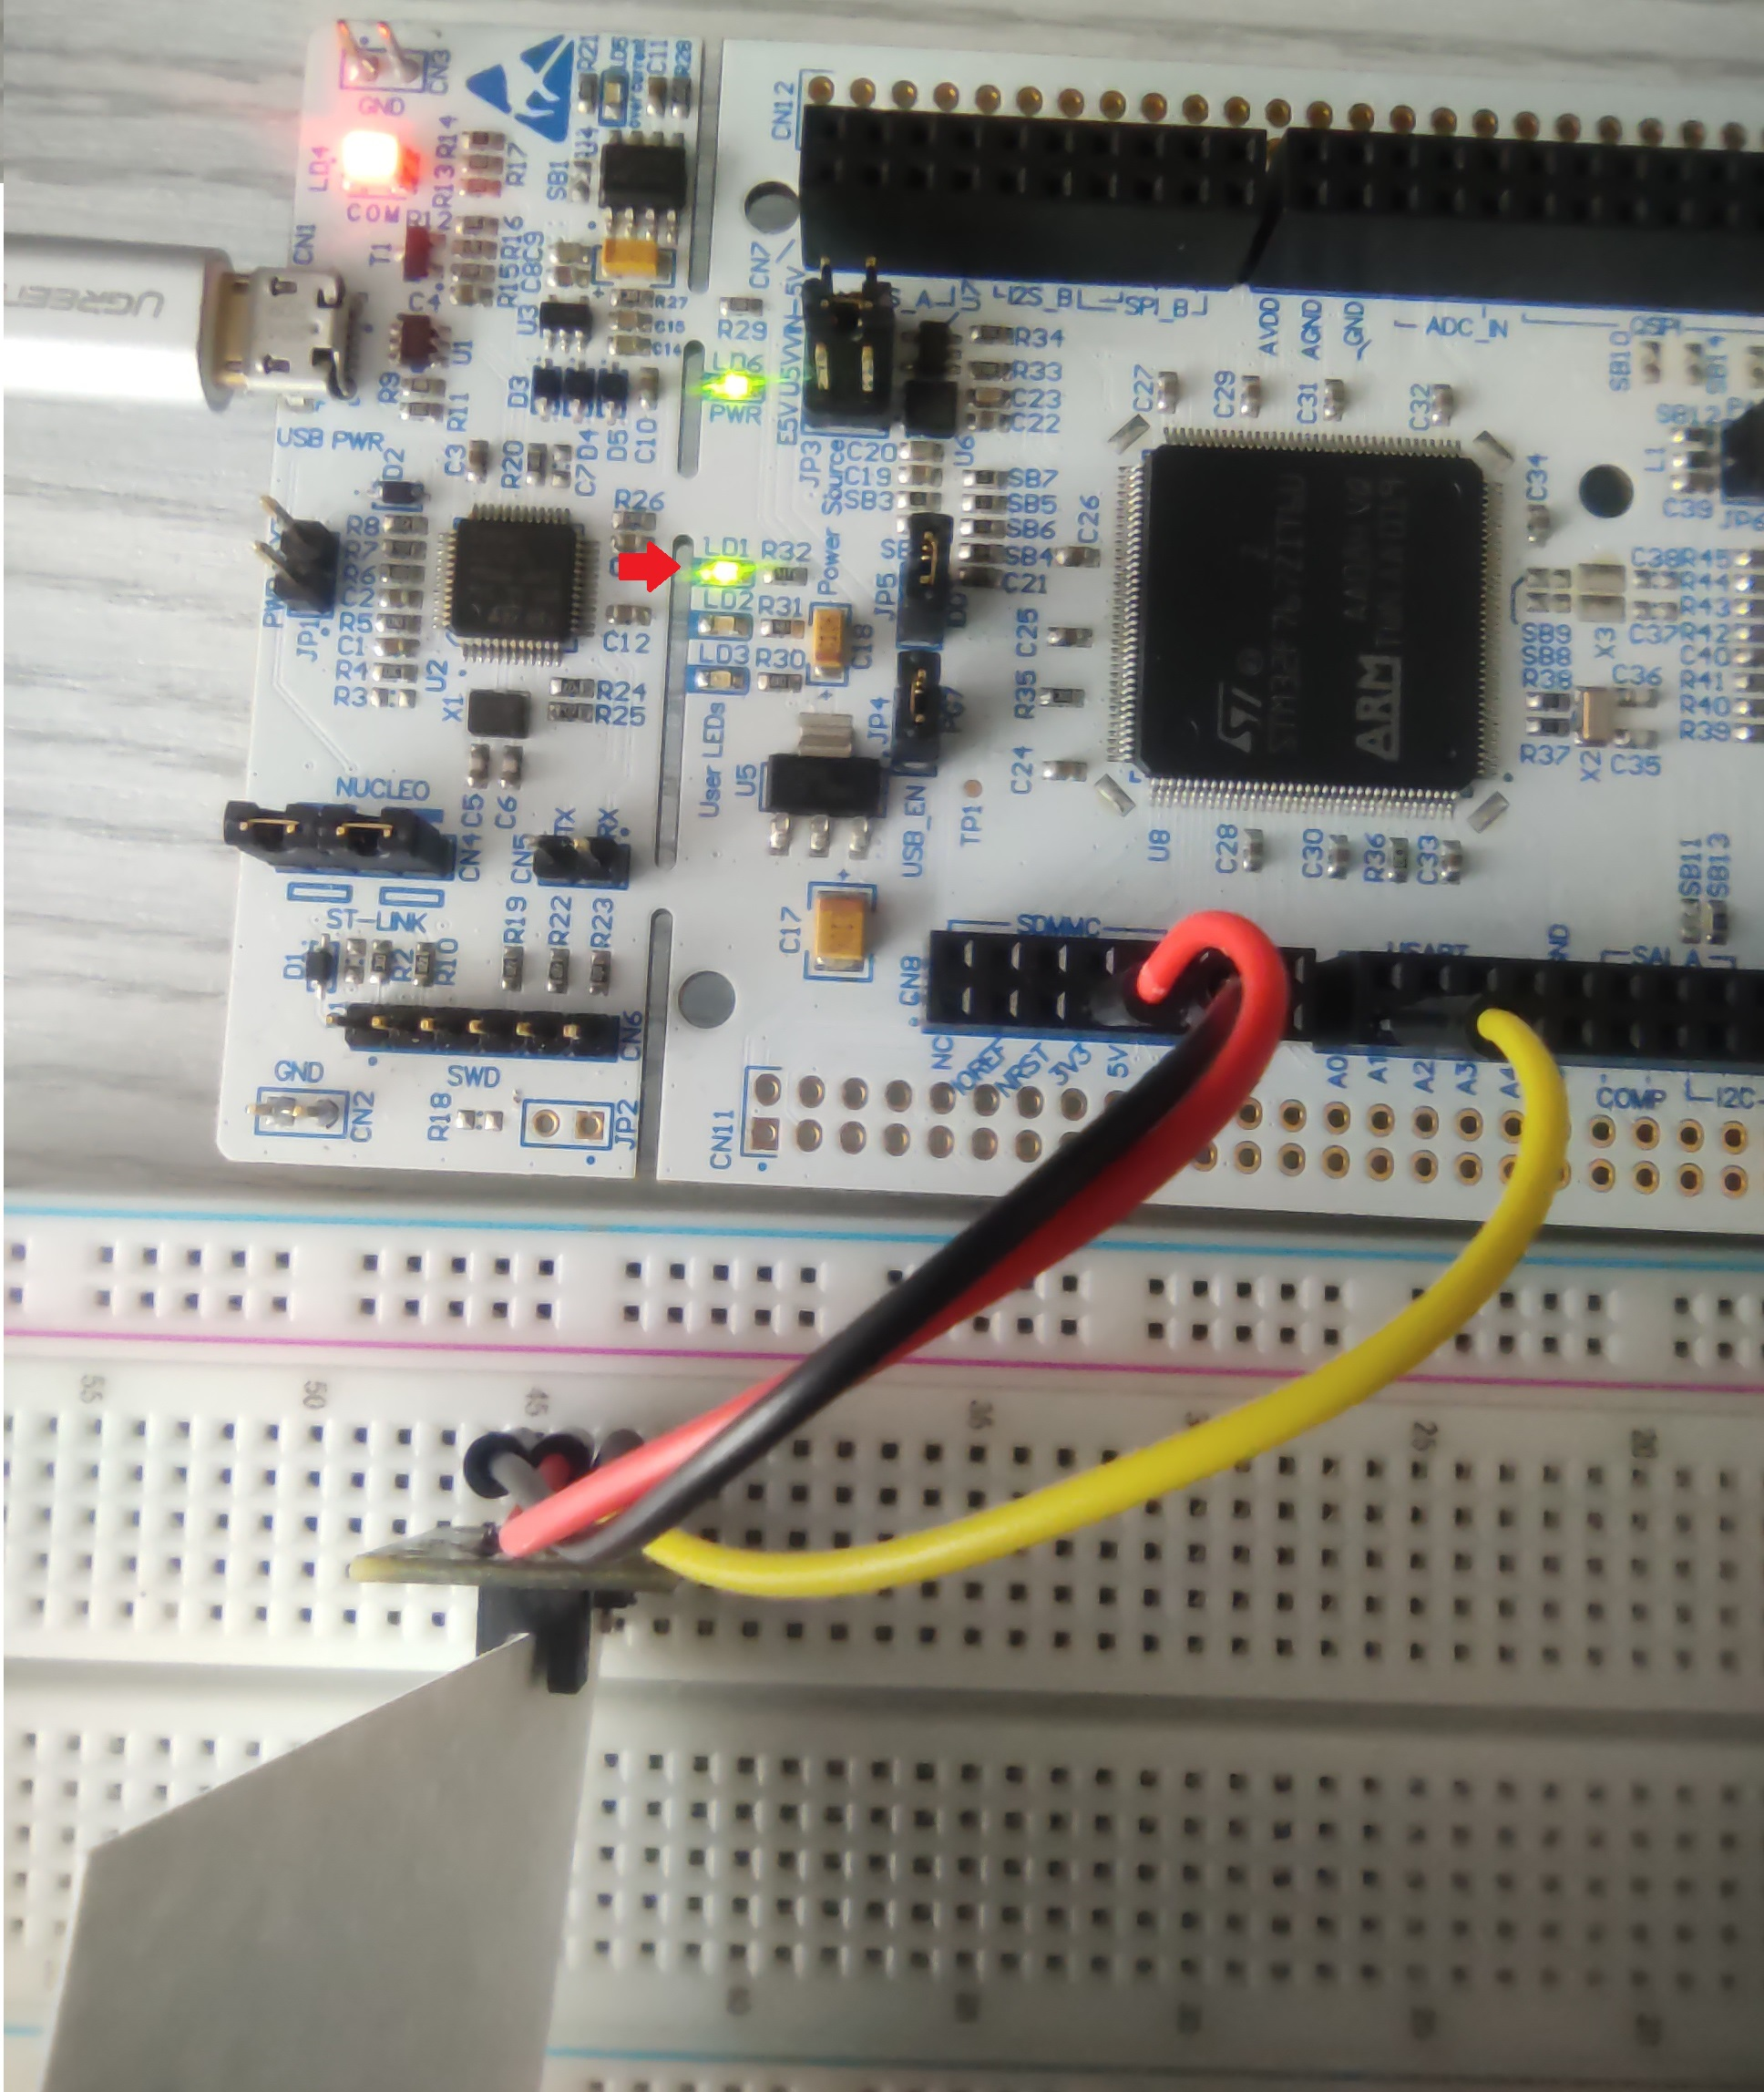
\includegraphics[width=.74\linewidth]{fig/HW-487/działanie_ukladu/led_on.jpg}
\caption{Szczelina zablokowana - stan wysoki na wyjściu S}
\label{fig:_uklad_on}
\end{subfigure}
%%%%%%%%%%%%%%%%%%%%%%%%%%%%%%%%%%%%%%%%%%%%%%%%%%%%%%%%%%%%%%%%%%%%%%%%%%%%%%%%%
% \caption{PODPIS}
\label{fig:mikroproc}
\end{figure}
\vspace{0.25cm}
%%%%%%%%%%%%%%%%%%%%%%%%%  TWO IMAGES SIDE BY SIDE  %%%%%%%%%%%%%%%%%%%%%%%%%%%%%
Dodatkowo działanie układu przedstawiono na załączonym w \texttt{Suplement Wideo} materiale 
wideo.

\newpage
\printbibliography[heading=bibintoc]

\end{document}